\chapter{Implementación Clásica: Algoritmo Word2Vec}

Word2Vec, cuyo nombre proviene de la contracción de \textit{Word to Vector}, es un modelo de \glsentrytext{ml} que permite representar palabras como vectores de grandes dimensiones. Su principal virtud reside en que las relaciones semánticas y sintácticas entre palabras quedan codificadas como proximidad geométrica entre dichos vectores, permitiendo así capturar el significado de forma numérica y operable.

Fue desarrollado y publicado por Google en 2013 \cite{google_word2vec_2013}, además en esa misma fecha, se introdujo este modelo en su motor de búsqueda. Desde entonces, el modelo ha sido ampliamente adoptado y ha dado lugar a múltiples mejoras y variantes de rendimiento.

En este capítulo se explorarán la arquitectura del modelo, su función de optimización y el proceso de entrenamiento que permite generar el espacio vectorial latente en el que las palabras quedan representadas.

\section{Arquitectura del modelo}

Word2Vec aprende las representaciones de las palabras procesando grandes volúmenes de texto y capturando el contexto en el que aparece cada término \cite{logunova_word2vec_serokell}. Su arquitectura se fundamenta en una red neuronal superficial (\textit{shallow neural network}), que a diferencia de las redes profundas (\textit{deep neural networks}), dispone únicamente de una capa oculta entre la capa de entrada y la de salida. Este diseño proporciona una ventaja clave: permite entrenar el modelo de forma eficiente sobre corpus de gran tamaño, manteniendo un coste computacional razonable.

\begin{figure}[h]
  \centering
  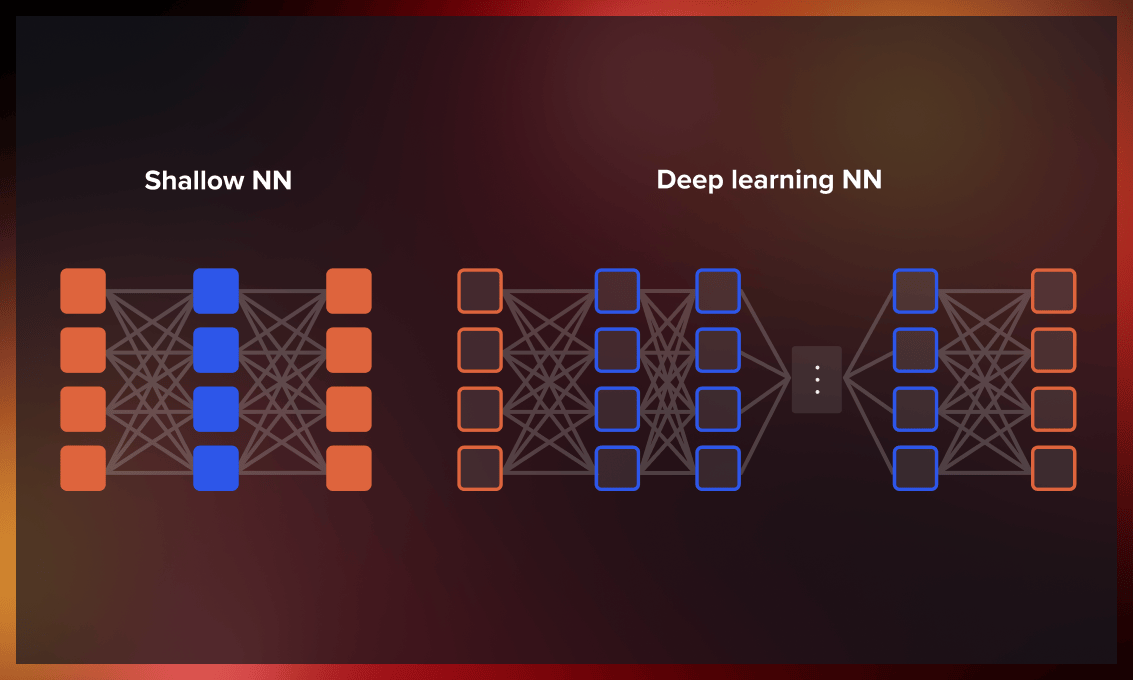
\includegraphics[width=0.8\linewidth]{imagenes/compRNNsWord2Vec.png}
  \caption{Comparativa entre una red neuronal superficial (Word2Vec) y una red neuronal profunda. Fuente: \cite{logunova_word2vec_serokell}.}
  \label{fig:comp_rnns_word2vec}
\end{figure}

El resultado del entrenamiento es la asignación de un vector de cientos de dimensiones a cada palabra del vocabulario. La posición de cada vector en ese espacio no es arbitraria, es decir, palabras empleadas en contextos similares acaban próximas entre sí, mientras que palabras semánticamente distantes se alejan geométricamente.

\begin{figure}[h]
  \centering
  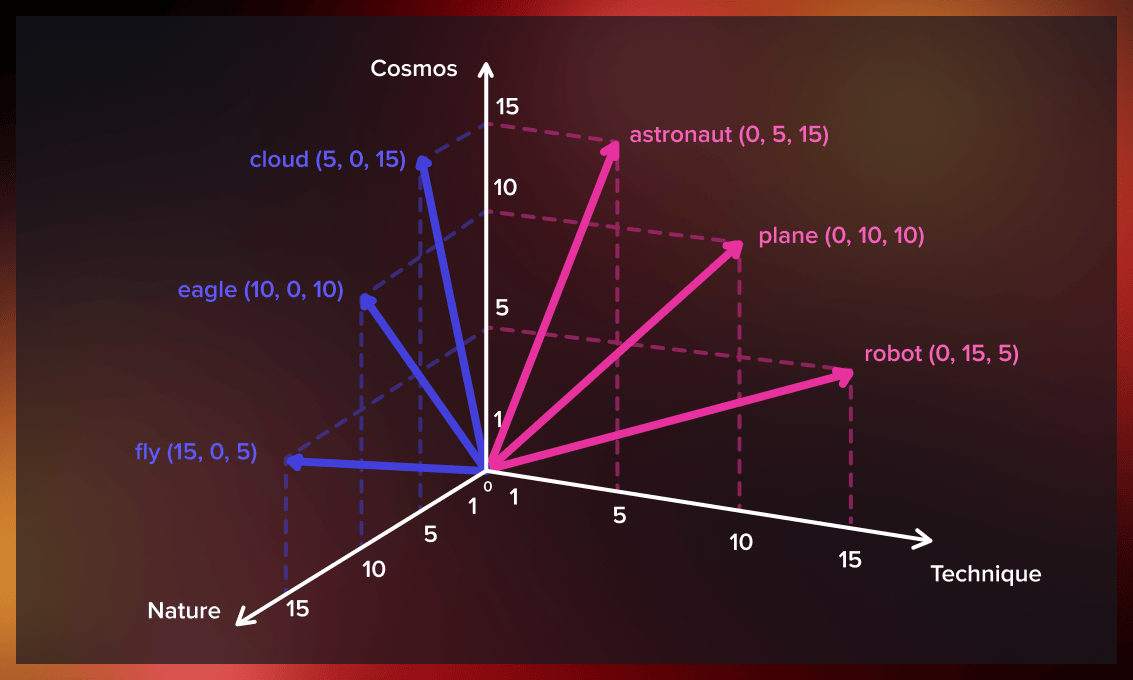
\includegraphics[width=0.8\linewidth]{imagenes/representacionWord2Vec.png}
  \caption{Representación vectorial de palabras en el espacio latente generado por Word2Vec. Fuente: \cite{logunova_word2vec_serokell}.}
  \label{fig:representacion_word2vec}
\end{figure}

Una consecuencia directa de esta estructura es que los vectores admiten operaciones algebraicas con significado semántico. El ejemplo más conocido de esta propiedad es la siguiente analogía entre género y realeza:

\[
  \vec{v}(\text{Rey}) - \vec{v}(\text{Hombre}) + \vec{v}(\text{Mujer}) \approx \vec{v}(\text{Reina})
\]

En esta expresión, al restar al vector de \textit{Rey} la componente que codifica la masculinidad y sumar la que codifica la feminidad, el vector resultante converge hacia la representación de \textit{Reina}. Esta propiedad es inherte a la forma natural del entrenamiento: como \textit{Rey} y \textit{Reina} comparten contextos de realeza pero difieren en los contextos de género, el modelo aprende implícitamente a separar ambas dimensiones dentro del espacio vectorial.

\begin{figure}[h]
  \centering
  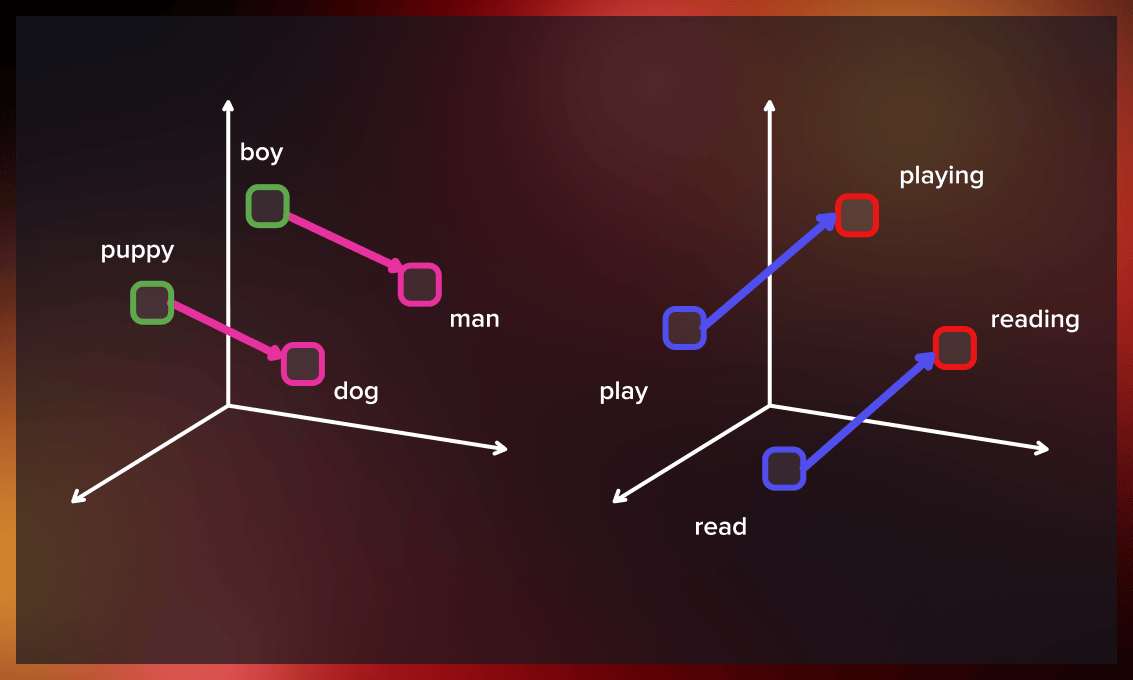
\includegraphics[width=0.8\linewidth]{imagenes/similitudesPalabrasWord2Vec.png}
  \caption{Representación geométrica de las similitudes semánticas entre palabras en el espacio vectorial de Word2Vec. Fuente: \cite{logunova_word2vec_serokell}.}
  \label{fig:similitudes_palabras_word2vec}
\end{figure}

\subsection{Modelos de entrenamiento: \glsentrytext{cbow} y Skip-gram}

Word2Vec ofrece dos variantes arquitectónicas para aprender los vectores de palabras: el modelo \textbf{\glsentrytext{cbow}} y el modelo \textbf{Skip-gram}. Ambos comparten la misma red neuronal superficial como base, pero se diferencian en el aprendizaje, qué se usa como entrada y qué se predice como salida.

En este trabajo se ha optado por implementar el modelo \textbf{Skip-gram}, ya que, como se verá en los capítulos siguientes, sus características lo hacen especialmente adecuado para la adaptación al entorno cuántico propuesto.

\subsubsection{Continuous Bag of Words (\glsentrytext{cbow})}

El modelo \glsentrytext{cbow} toma como entrada las palabras del contexto que rodean a una posición central y predice cuál es la palabra que debería ocupar dicha posición. En otras palabras, dadas las palabras vecinas, el modelo intenta adivinar la palabra central.

\begin{figure}[h]
  \centering
  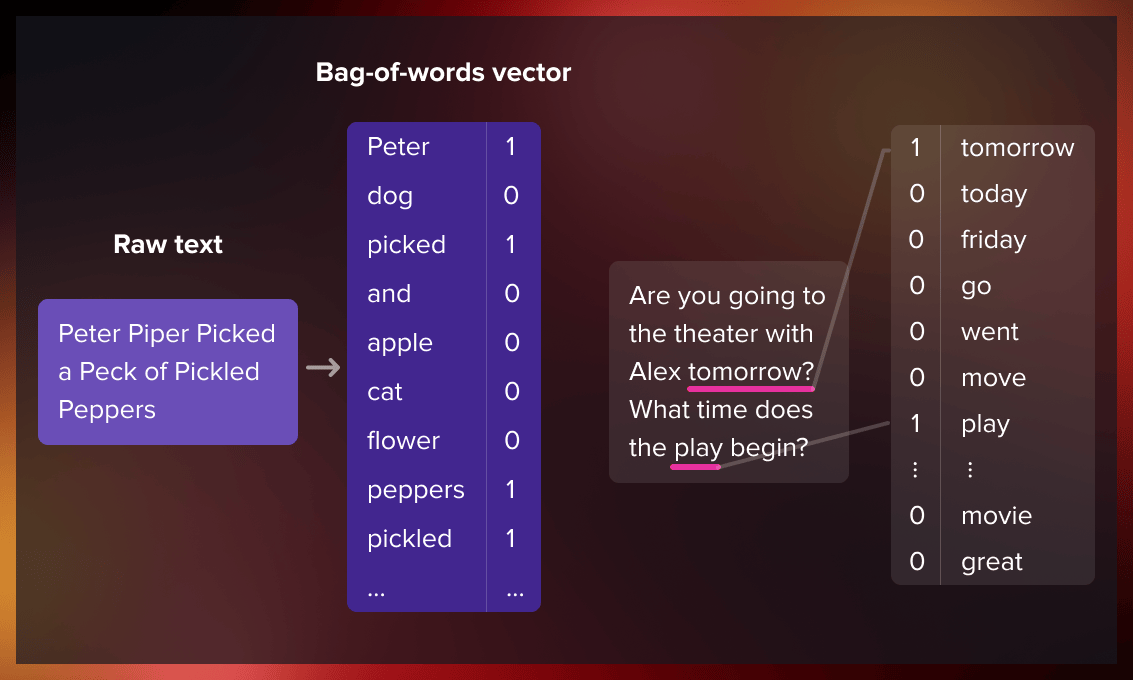
\includegraphics[width=0.8\linewidth]{imagenes/bowExample.png}
  \caption{Ejemplo del funcionamiento del modelo \glsentrytext{cbow}: a partir de las palabras de contexto circundantes se predice la palabra objetivo central. Fuente: \cite{logunova_word2vec_serokell}.}
  \label{fig:cbow_example}
\end{figure}

Este enfoque resulta eficiente cuando el corpus es grande y las palabras frecuentes tienen representaciones ricas. Sin embargo, tiende a promediar la información del contexto, lo que puede penalizar los valores semánticos de palabras menos frecuentes.

\subsubsection{Skip-gram}

Skip-gram es un modelo diseñado para hacer lo opuesto a \glsentrytext{cbow}. En lugar de predecir la palabra central a partir del contexto que tiene en su ventana, toma una única palabra central como entrada e intenta predecir las palabras que aparecen a su alrededor.

El proceso de entrenamiento de esta red neuronal superficial funciona de la siguiente manera: dada la palabra central (la palabra de entrada), se selecciona aleatoriamente una palabra de su contexto inmediato. La red calcula cuál es la probabilidad de que cada palabra del vocabulario sea una palabra "cercana" a la palabra de entrada \cite{mccormick_skipgram_2016}.

Los resultados de estas probabilidades indican cuán probable es que cada término del vocabulario aparezca en las proximidades de la palabra de entrada. Por ejemplo, si la palabra de entrada proporcionada a la red ya entrenada es \textit{reino}, las probabilidades serán considerablemente mayores para palabras como \textit{España} o \textit{Inglaterra} que para términos sin relación semántica como \textit{lápiz} o \textit{mango}.

\subsubsection{Detalles del modelo básico Skip-gram}

Dado que una red neuronal no puede procesar cadenas de texto directamente, cada palabra se representa mediante un \textit{vector one-hot} (una forma de codificación sencilla aunque no la única). Consiste en un vector de tantas componentes como palabras tiene el vocabulario (por ejemplo, 10.000), donde únicamente la posición correspondiente a la palabra de entrada vale 1 y el resto valen 0.

La capa de salida de la red produce también un vector de 10.000 componentes, donde cada valor refleja la probabilidad de que la palabra correspondiente sea una palabra cercana a la entrada. No existe función de activación en la capa oculta, pero la capa de salida aplica \textit{softmax} para normalizar las probabilidades.

\begin{figure}[h]
  \centering
  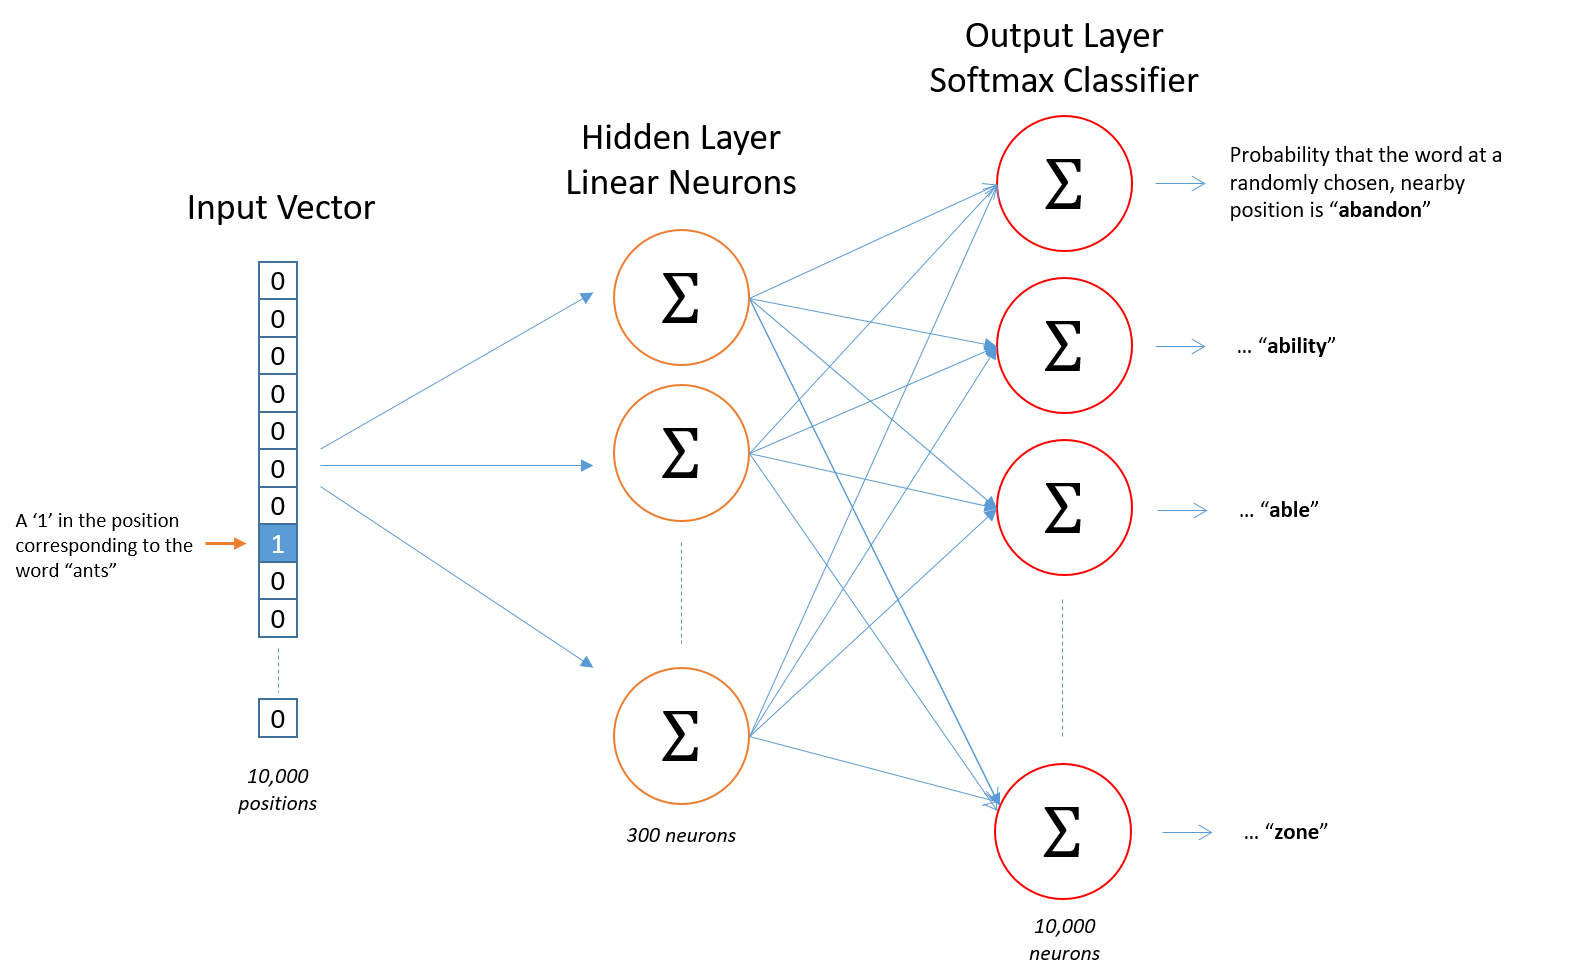
\includegraphics[width=0.7\linewidth]{imagenes/redSkipGram.png}
  \caption{Arquitectura de la red neuronal del modelo Skip-gram. Fuente: \cite{mccormick_skipgram_2016}.}
  \label{fig:red_skip_gram}
\end{figure}

Durante el entrenamiento, tanto la entrada como la salida de la red son vectores \textit{one-hot}. Sin embargo, al evaluar la red con una palabra de entrada, el vector de salida ya no es \textit{one-hot}, sino una distribución de probabilidad sobre todo el vocabulario.

A modo de ejemplo concreto, supóngase que la \textbf{capa oculta} aprende vectores de palabras de 300 dimensiones. En ese caso, los pesos de dicha capa quedan representados por una matriz de $10.000 \times 300$: una fila por cada palabra del vocabulario y una columna por cada neurona oculta. Este es precisamente el tamaño que empleó Google en el trabajo original en el que presentó Word2Vec \cite{google_word2vec_2013}.

Al final, el objetivo de este modelo es aprender la matriz de pesos de la capa oculta. Una vez se tiene esta matriz, la capa de salida es inmediata.

\begin{figure}[h]
  \centering
  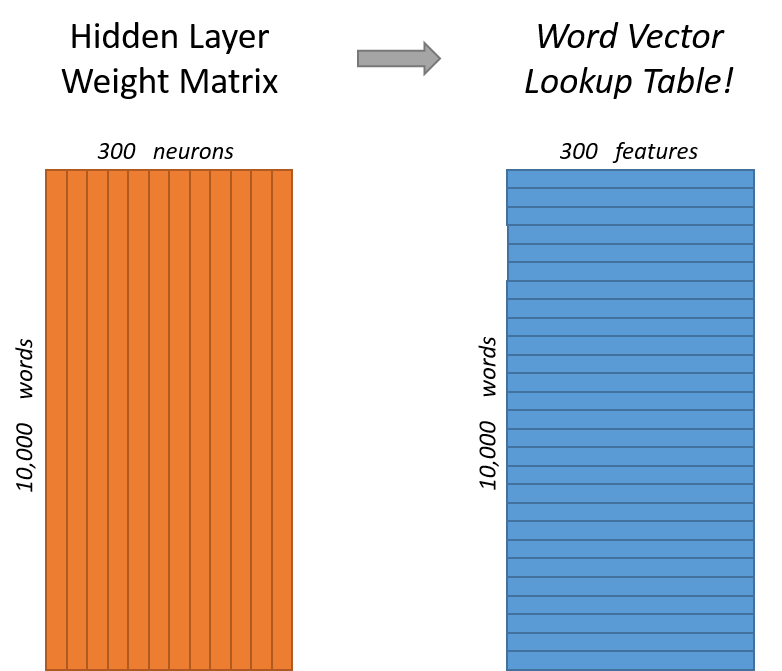
\includegraphics[width=0.6\linewidth]{imagenes/matrizPesosSkipGram.png}
  \caption{Matriz de pesos de la capa oculta del modelo Skip-gram: 10.000 filas (una por palabra del vocabulario) y 300 columnas (una por neurona oculta). Cada fila constituye el vector de representación de su palabra correspondiente. Fuente: \cite{mccormick_skipgram_2016}.}
  \label{fig:matriz_pesos_skip_gram}
\end{figure}

Llegados a este punto, uno puede preguntarse cuál es la utilidad de representar las palabras mediante vectores de todo ceros salvo una única posición con valor $1$. La respuesta reside en la eficiencia, multiplicar un vector \textit{one-hot} de $1 \times 10.000$ por la matriz de $10.000 \times 300$ selecciona de forma inmediata la fila correspondiente a la palabra de entrada, sin necesidad de realizar el producto matricial completo.

\begin{figure}[h]
  \centering
  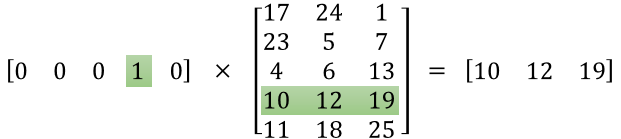
\includegraphics[width=0.7\linewidth]{imagenes/multMatrizOneHot.png}
  \caption{Multiplicación de un vector \textit{one-hot} por la matriz de pesos de la capa oculta, obteniendo directamente el vector de representación de la palabra de entrada. Fuente: \cite{mccormick_skipgram_2016}.}
  \label{fig:mult_matriz_one_hot}
\end{figure}

Con esto se concluye que la capa oculta del modelo actúa en realidad como una tabla \textit{lookup}: la salida de dicha capa es directamente el vector de representación de la palabra de entrada. Así, el vector de $1 \times 300$ resultante se pasa a la \textbf{capa de salida}, que es un clasificador de regresión \textit{softmax}.

Cada neurona de salida produce un valor entre 0 y 1 aplicando la función $\exp(x)$ sobre el producto de su vector de pesos y el vector proveniente de la capa oculta. Para que todos los valores sumen 1 y formen una distribución de probabilidad, cada resultado se divide entre la suma de los valores de las 10.000 neuronas de salida \cite{mccormick_skipgram_2016}.

\begin{figure}[h]
  \centering
  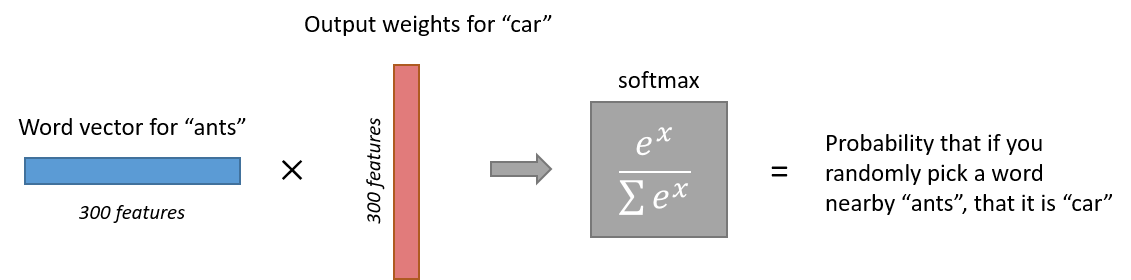
\includegraphics[width=0.9\linewidth]{imagenes/ejemploCapaSalidaSkipGram.png}
  \caption{Cálculo de la salida de la neurona correspondiente a la palabra \textit{car} en la capa \textit{softmax} del modelo Skip-gram. Fuente: \cite{mccormick_skipgram_2016}.}
  \label{fig:ejemplo_capa_salida_skip_gram}
\end{figure}

\section{Función de optimización y pérdida}

\section{Entrenamiento y generación del espacio latente}

